\documentclass[12pt]{article}
\usepackage[utf8]{inputenc}
\usepackage{float}
\usepackage{amsmath}
%\usepackage{amssymb}

\usepackage[hmargin=3cm,vmargin=6.0cm]{geometry}
%\topmargin=0cm
\topmargin=-2cm
\addtolength{\textheight}{6.5cm}
\addtolength{\textwidth}{2.0cm}
%\setlength{\leftmargin}{-5cm}
\setlength{\oddsidemargin}{0.0cm}
\setlength{\evensidemargin}{0.0cm}

%misc libraries goes here
\usepackage{tikz}
\usetikzlibrary{automata,positioning,shapes}

\begin{document}

\section*{Student Information } 
%Write your full name and id number between the colon and newline
%Put one empty space character after colon and before newline
Full Name :  Onur Can TIRTIR\\
Id Number :  2099380\\

% Write your answers below the section tags
\section*{Answer 1}

\subsection*{a.}
Here is our automata:
\begin{center}
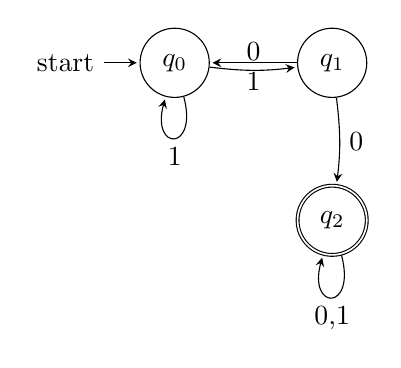
\begin{tikzpicture}
	[>= stealth, shorten >= 1pt,node distance = 2cm,on grid,auto]
\node[state,initial](q_0){$q_0$};
\node[state](q_1)[right = of q_0]{$q_1$};
\node[state,accepting](q_2)[below = of q_1]{$q_2$};

\path[->]  
	(q_2)	edge [loop below] node{0,1} ()
	(q_1)   edge [bend left =7] node {0} (q_2)
	(q_1)   edge node {1} (q_0)
	(q_0)   edge [bend right =7] node {0} (q_1)
	(q_0)	edge [loop below] node{1} ();

\end{tikzpicture}
\end{center}
Then the transitions for the string $1011011$ in our automata is as below:
\begin{align*}
	(q_0, 11011011) & \vdash_M (q0, 1011011) \\
				    & \vdash_M (q1, 011011) \\
				    & \vdash_M (q0, 11011) \\
				    & \vdash_M (q0, 1011) \\
				    & \vdash_M (q1, 011) \\
				    & \vdash_M (q2, 11) \\
				    & \vdash_M (q2, 1) \\
				    & \vdash_M (q2, e)
\end{align*}
Then the string given above belongs to $L_1$.

\subsection*{b.}
\begin{center}
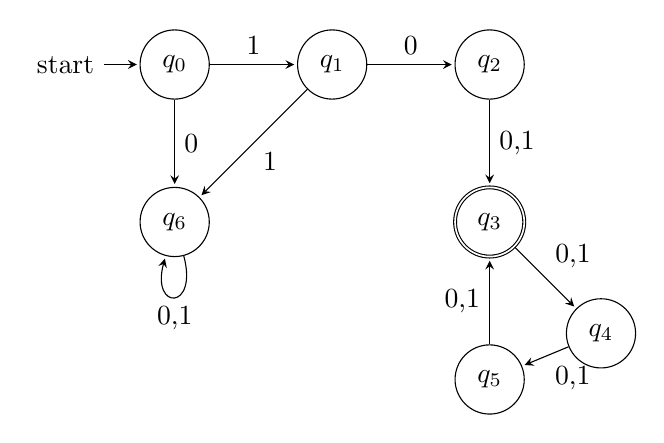
\begin{tikzpicture}
	[>= stealth, shorten >= 1pt,node distance = 2cm,on grid,auto]
\node[state,initial](q_0){$q_0$};
\node[state](q_1)[right = of q_0]{$q_1$};
\node[state](q_2)[right = of q_1]{$q_2$};
\node[state, accepting](q_3)[below = of q_2]{$q_3$};
\node[state](q_4)[below right = of q_3]{$q_4$};
\node[state](q_5)[below = of q_3]{$q_5$};
\node[state](q_6)[below = of q_0]{$q_6$};

\path[->]  
	(q_0)	edge node {1} (q_1)
	(q_0)	edge node {0} (q_6)
	(q_1)	edge node {0} (q_2)
	(q_1)	edge node {1} (q_6)
	(q_2)	edge node {0,1} (q_3)
	(q_3)	edge node {0,1} (q_4)
	(q_4)	edge node {0,1} (q_5)
	(q_5)	edge node {0,1} (q_3) 
	(q_6)	edge [loop below] node{0,1} ();
\end{tikzpicture}
\end{center}

Then the transitions for the string $1000111$ in our automata is as below:
\begin{align*}
	(q_0, 1000111)  & \vdash_M (q1, 000111) \\
				    & \vdash_M (q2, 00111) \\
				    & \vdash_M (q3, 0111) \\
				    & \vdash_M (q4, 111) \\
				    & \vdash_M (q5, 11) \\
				    & \vdash_M (q3, 1) \\
				    & \vdash_M (q4, e) \\
\end{align*}
Then the string given above was consumed but $q_4$ was not a \textit{final state}. Then this string does not belong to $L_2$.

\section*{Answer 2}

$L_3=1^*0(1\cup 0)^*0(1\cup 0)^*1$

\section*{Answer 3}

\subsection*{a.}

\textit{Countable.}\\

Take the finite alphabet $\Sigma$ and say $Q$ is the set of states of our automaton. We know for any finite alphabet, $Kleene\ Star$ is countably infinite by definition then $\Sigma^*$ is also countably infinite. Also we know that $\Sigma^*$ is the set of all strings over $\Sigma$.\\

Since we are talking about a \textit{"finite"} automaton then $Q$ is finite.\\

$Configurations$ within an automata over these strings are of the form $(q_i, w_k)$ where $q_i\in Q$ and $w_k\in \Sigma_{}^*$, so $(q_i, w_k) \in Q \times \Sigma_{}^*$. Since $Q$ is finite and $\Sigma_{}^*$ is countable then their cartesian product is also countable. Hence set of configurations of a finite automaton on all strings over $\Sigma_{}$ is countable because it is a subset of $Q \times \Sigma_{}^*$ (\textit{Note: This is because it is not a necessary that every string matches with every state.}). As a result, it is the same as saying that \textit{"the set of configurations of a finite automaton on all strings over finite alphabet is countable."}

\subsection*{b.}

\textbf{Note: }If number of symbols in universe is assumed to uncountable, then the answer will be uncountable since in this case strings over this uncountable set is also uncountable and so all finite automatons on these strings are. Hence configurations of all these finite automatons are also uncountable since in this case configurations will be from a cartesian product, one of which contributing this cartesian product is an uncountable set.\\

\textit{Countable.}\\

We know number of regular expressions on a language over a finite alphabet is countably inifinite \textbf{(see (*)1 below)}. Also we know for any automaton, we have only one corresponding regular expression over this language. Since regular expression are countable and there exists a $1-1$ correspondance between regular expressions and finite automatas over a certain language, then we can count finite automatas. We have already proven that we could count the number of configurations of \textbf{"a"} finite automata on all strings over all possible finite alphabets \textbf{(see (*)2) below}. Our finite automatas are countably infinite. Hence we can say that \textit{"the set of configurations of all finite automatons on all strings over all possible finite alphabets is countable."}\\

\textbf{(*1)}
Regular expressions over a finite alphabet $\Sigma$ is just \textit{Kleene Star} of a finite set of symbols such that $$\Sigma \cup \{\cup, *, (, )\}$$.

\textbf{(*2)}
1) \textbf{Assuming that the number of symbols in universe, which can be used to create an alphabet, is finite}, number of possible finite alphabets are countable since alphabets are subsets of symbols. Say we have $n$ many different alphabets.
Assume a new alphabet $\Sigma_{new}$ and say $\Sigma_{new}=\cup_{i=1}^n \Sigma_i$ where every $\Sigma_i$ is representing a possible alphabet in the universe. So $\Sigma_{new}$ is finite since it is the construction of finite number of unions of finite alphabets. Also note that $\Sigma_{new}^*=\cup_{i=1}^n \Sigma_i^*$. This is because if we sort the alphabets $\Sigma_i$ from smaller to larger cardinality, then we can say $\Sigma_n=\Sigma$. Also, the strings over other smaller alphabets $\Sigma_i^*$ are already included in $\Sigma_n^*$ since $\Sigma_i^*=(\cup_{k=1}^i \alpha_k)^* \subseteq (\cup_{k=1}^n \alpha_k)^* = \Sigma_n^*$ where each $\alpha$ represents a symbol. \\

We know for any finite alphabet, $\Sigma^*$ is countably infinite by definition then $\Sigma_{new}^*$ is also countably infinite. Also we know that $\Sigma^*$ is the set of all strings over $\Sigma$.\\

2) Since we are talking about a \textit{"finite"}, automaton then $Q$ is finite.\\

$Configurations$ within an automata over these strings are of the form $(q_i, w_k)$ where $q_i\in Q$ and $w_k\in \Sigma_{new}^*$, so $(q_i, w_k) \in Q \times \Sigma_{new}^*$. Since $Q$ is finite and $\Sigma_{new}^*$ is countable then their cartesian product is also countable. Hence set of configurations of a finite automaton on all strings over $\Sigma_{new}$ is countable because it is a subset of $Q \times \Sigma_{new}^*$ (\textit{Note: This is because it is not a necessary that every string matches with every state.}). As a result, it is the same as saying that \textit{"the set of configurations of a finite automaton on all strings over all possible finite alphabets is countable."}\\

\section*{Answer 4}

\subsection*{a.}

\begin{align*}
	E(q_0) & = {q_0} \\
	E(q_1) & = {q_1, q_4} \\
	E(q_2) & = {q_2} \\
	E(q_3) & = {q_3, q_4} \\
	E(q_4) & = {q_4} 
\end{align*}
Where $E(q_0)=q_0$ will be our starting node. Also we can say that if we have $E(q_4)=q_4$ in a subset in DFA, then this subset is one of the accepting states.\\

\begin{align*}
	\delta^{'} (\{q_0\}, a) & = E(q_0) \cup E(q_3) & = \{q_0, q_3, q_4\} \\
	\delta^{'} (\{q_0\}, b) & = E(q_1) & = \{q_1, q_4\} \\
	\delta^{'} (\{q_0, q_3, q_4\}, a) & = E(q_0) \cup E(q_3) & = \{q_0, q_3, q_4\} \\
	\delta^{'} (\{q_0, q_3, q_4\}, b) & = E(q_0) \cup E(q_1) & = \{q_0, q_1, q_4\} \\
	\delta^{'} (\{q_1, q_4\}, a) & = E(q_2) & = \{q_2\} \\
	\delta^{'} (\{q_1, q_4\}, b) & = E(q_1) \cup E(q_2) & = \{q_1, q_2, q_4\} \\
	\delta^{'} (\{q_0, q_1, q_4\}, a) & = E(q_0) \cup E(q_2) \cup E(q_3) & = \{q_0, q_2, q_3, q_4\} \\
	\delta^{'} (\{q_0, q_1, q_4\}, b) & = E(q_1) \cup E(q_2) & = \{q_1, q_2, q_4\} \\
	\delta^{'} (\{q_2\}, a) & = E(q_3) & = \{q_3, q_4\} \\
	\delta^{'} (\{q_2\}, b) & = E(q_0) & = \{q_0\} \\
	\delta^{'} (\{q_1, q_2, q_4\}, a) & = E(q_2) \cup E(q_3) & = \{q_2, q_3, q_4\} \\
	\delta^{'} (\{q_1, q_2, q_4\}, b) & = E(q_0) \cup E(q_1) \cup E(q_2) & = \{q_0, q_1, q_2, q_4\} \\
	\delta^{'} (\{q_0, q_2, q_3, q_4\}, a) & = E(q_0) \cup E(q_3) & = \{q_0, q_3, q_4\} \\
	\delta^{'} (\{q_0, q_2, q_3, q_4\}, b) & = E(q_0) \cup E(q_1) & = \{q_0, q_1, q_4\} \\
	\delta^{'} (\{q_3, q_4\}, a) & = \{\} & = \{\} \\
	\delta^{'} (\{q_3, q_4\}, b) & = E(q_0) & = \{q_0\} \\
	\delta^{'} (\{q_2, q_3, q_4\}, a) & = E(q_3) & = \{q_3, q_4\} \\
	\delta^{'} (\{q_2, q_3, q_4\}, b) & = E(q_0) & = \{q_0\} \\
	\delta^{'} (\{q_0, q_1, q_2, q_4\}, a) & = E(q_0) \cup E(q_2) \cup E(q_3) & = \{q_0, q_2, q_3, q_4\} \\
	\delta^{'} (\{q_0, q_1, q_2, q_4\}, b) & = E(q_0) \cup E(q_1) & = \{q_0, q_1, q_4\}
\end{align*}

\begin{center}
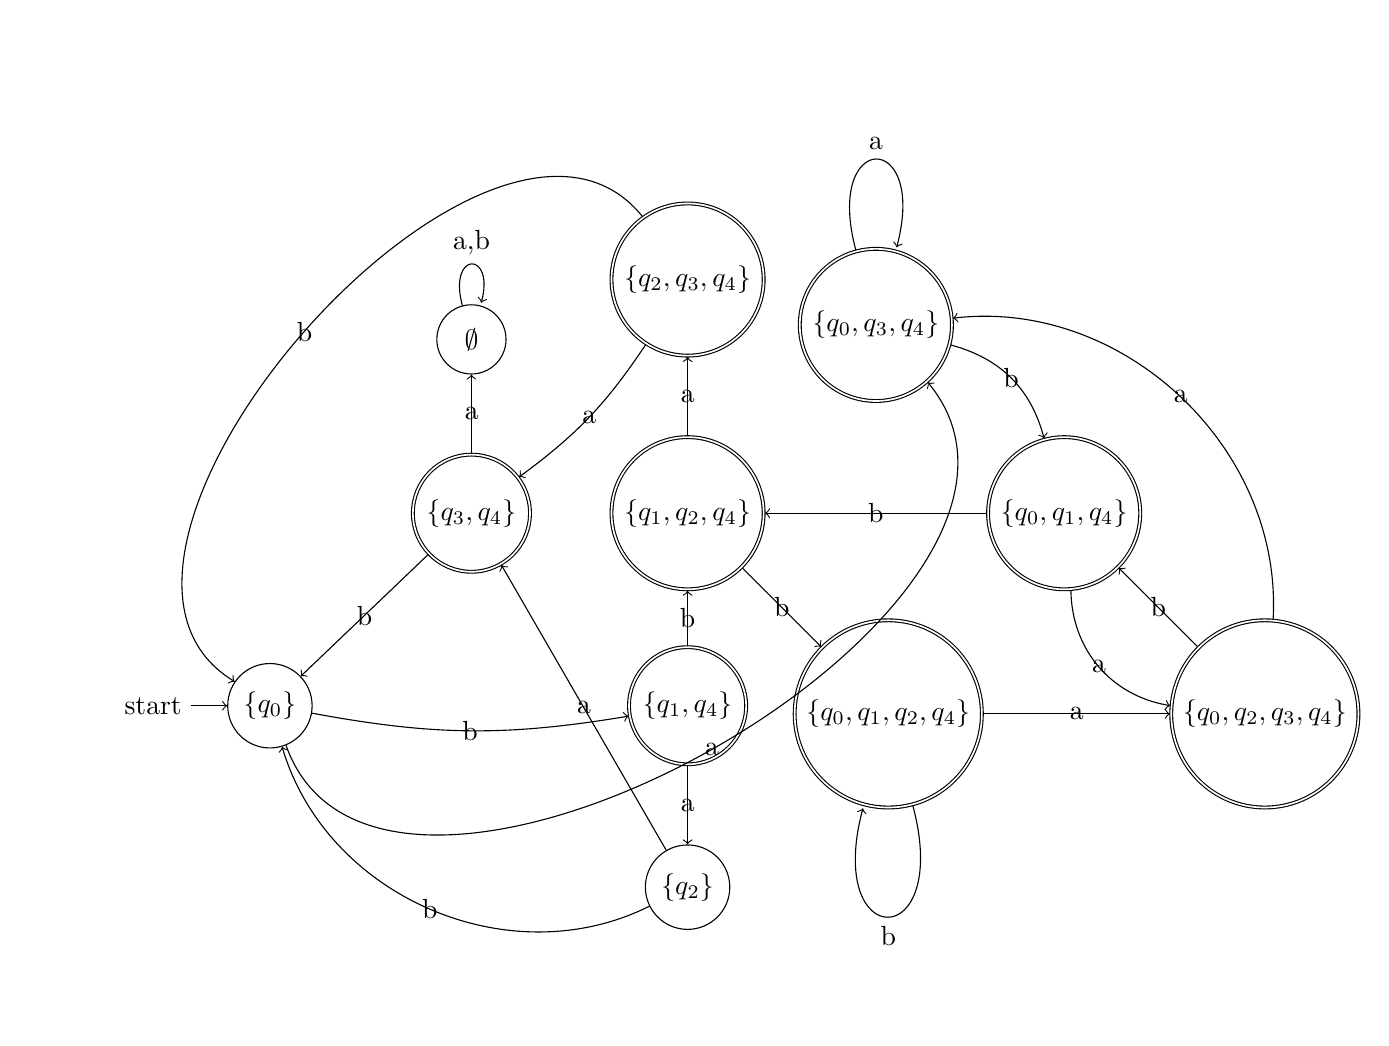
\begin{tikzpicture}
\node[state, accepting](4){$\{q_1, q_4\}$};
\node[state, initial](2)[left = 4.0cm of 4]{$\{q_0\}$};
\node[state](3)[below = of 4]{$\{q_2\}$};
\node[state, accepting](5)[above = 0.7cm of 4]{$\{q_1, q_2, q_4\}$};
\node[state, accepting](1)[left = of 5]{$\{q_3, q_4\}$};
\node[state, accepting](6)[above = of 5]{$\{q_2, q_3, q_4\}$};
\node[state, accepting](7)[above right = of 5]{$\{q_0, q_3, q_4\}$};
\node[state, accepting](8)[below right = of 7]{$\{q_0, q_1, q_4\}$};
\node[state, accepting](9)[below right = of 8]{$\{q_0, q_2, q_3, q_4\}$};
\node[state, accepting](11)[below right = of 5]{$\{q_0, q_1, q_2, q_4\}$};
\node[state](10)[above = of 1]{$\emptyset$};

\path[->]  
	(3)	edge [bend left=50] node {b} (2)
	(4)	edge node {a} (3)
	(4)	edge node {b} (5)
	(5)	edge node {a} (6)
	(6)	edge [bend left=10] node {a} (1)
	(1)	edge node {a} (10)
	(1) edge node {b} (2)
	(5) edge node {b} (11)
	(8) edge node {b} (5)
	(7) edge [bend left=30] node {b} (8)
	(8) edge [bend right=40] node {a} (9)
	(9) edge node {b} (8)
	(9) edge [bend right=50] node {a} (7)
	(3) edge node {a} (1)
	(2) edge [bend right=10] node {b} (4)
	(6) edge [bend right=100] node {b} (2)
	(2) edge [bend right=100] node {a} (7)
	(11) edge node {a} (9)
	(7) edge [loop above] node{a} ()
	(10) edge [loop above] node{a,b} ()
	(11) edge [loop below] node{b} ();
\end{tikzpicture}
\end{center}

\subsection*{b.}

Since $empty$ string cannot be accepted by our language, then we should include it by concataneting $L$ to $L^*$ such that $L^+=LL^*$. Also, we can find $L$ by sequentially removals of paths. At the end, we have only two states, some loops and some paths which are connecting starting state with accepting state.
$$\big([bb^*(a\cup b)b\cup bb^*(a\cup b)ab\cup a(b\cup \emptyset)]^*(bb^*(\emptyset\cup(a\cup b)a)\cup a\big)\big([bb^*(a\cup b)b\cup bb^*(a\cup b)ab\cup a(b\cup \emptyset)]^*(bb^*(\emptyset\cup(a\cup b)a)\cup a)\big)^*$$

\subsection*{c.}

We should first reverse edges. Also we should make $q_0$ accepting node and $q_4$ initial node. Then we can change the odtained NFA to DFA by subset construction algorithm.\\

Now apply subset construction algorithm.

\begin{align*}
	E(q_0) & = \{q_0\} \\ 
	E(q_1) & = \{q_1\} \\
	E(q_2) & = \{q_2\} \\
	E(q_3) & = \{q_3\} \\
	E(q_4) & = \{q_1, q_3, q_4\} \\
\end{align*}

Where $E(q_4)=\{q_1, q_3, q_4\}$ will be our starting node. Also we can say that if we have $E(q_0)=q_0$ in a subset in DFA, then this subset is one of the accepting states.\\

\begin{align*}
	\delta^{'} (\{q_1, q_3, q_4\}, a) & = E(q_0) \cup E(q_2) & = \{q_0, q_2\} \\
	\delta^{'} (\{q_1, q_3, q_4\}, b) & = E(q_1) \cup E(q_0) & = \{q_0, q_1\} \\
	\delta^{'} (\{q_0, q_2\}, a) & = E(q_0) \cup E(q_1) & = \{q_0, q_1\} \\
	\delta^{'} (\{q_0, q_2\}, b) & = E(q_1) \cup E(q_2) \cup E(q_3) & = \{q_1, q_2, q_3\} \\
	\delta^{'} (\{q_0, q_1\}, a) & = E(q_0) & = \{q_0\} \\
	\delta^{'} (\{q_0, q_1\}, b) & = E(q_0) \cup E(q_1) \cup E(q_2) \cup E(q_3) & = \{q_0, q_1, q_2, q_3\} \\
	\delta^{'} (\{q_1, q_2, q_3\}, a) & = E(q_0) \cup E(q_1) \cup E(q_2) & = \{q_0, q_1, q_2\} \\
	\delta^{'} (\{q_1, q_2, q_3\}, b) & = E(q_0) \cup E(q_1) & = \{q_0, q_1\} \\
	\delta^{'} (\{q_0\}, a) & = E(q_0) & = \{q_0\} \\
	\delta^{'} (\{q_0\}, b) & = E(q_2) \cup E(q_3) & = \{q_2, q_3\} \\
	\delta^{'} (\{q_0, q_1, q_2, q_3\}, a) & = E(q_0) \cup E(q_1) \cup (q_2) & = \{q_0, q_1, q_2\} \\
	\delta^{'} (\{q_0, q_1, q_2, q_3\}, b) & = E(q_0) \cup E(q_1) \cup E(q_2) \cup E(q_3) & = \{q_0, q_1, q_2, q_3\} \\
	\delta^{'} (\{q_0, q_1, q_2\}, a) & = E(q_0) \cup E(q_1) & = \{q_0, q_1\} \\
	\delta^{'} (\{q_0, q_1, q_2\}, b) & = E(q_0) \cup E(q_1) \cup E(q_2) \cup E(q_3) & = \{q_0, q_1, q_2, q_3\} \\
	\delta^{'} (\{q_2, q_3\}, a) & = E(q_0) \cup E(q_1) \cup E(q_2) & = \{q_0, q_1, q_2\} \\
	\delta^{'} (\{q_2, q_3\}, b) & = E(q_1) & = \{q_1\} \\
	\delta^{'} (\{q_0, q_1, q_2\}, a) & = E(q_0) \cup E(q_1) & = \{q_0, q_1\} \\
	\delta^{'} (\{q_0, q_1, q_2\}, b) & = E(q_0) \cup E(q_1) \cup E(q_2) \cup E(q_3) & = \{q_0, q_1, q_2, q_3\} \\
	\delta^{'} (\{q_1\}, a) & = \emptyset & = \emptyset \\
	\delta^{'} (\{q_1\}, b) & = E(q_0) \cup E(q_1) & = \{q_0, q_1\} \\
\end{align*}

\begin{center}
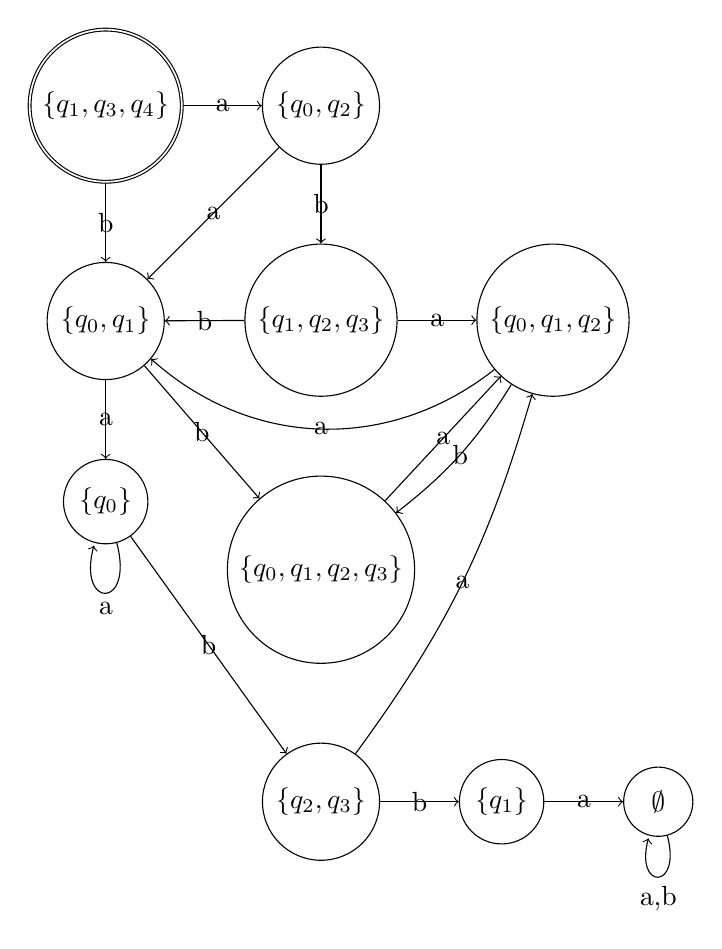
\begin{tikzpicture}
\node[state, accepting](0){$\{q_1, q_3, q_4\}$};
\node[state](2)[below = of 0]{$\{q_0, q_1\}$};
\node[state](4)[below = of 2]{$\{q_0\}$};
\node[state](1)[right = of 0]{$\{q_0, q_2\}$};
\node[state](3)[below = of 1]{$\{q_1, q_2, q_3\}$};
\node[state](5)[below = of 3]{$\{q_0, q_1, q_2, q_3\}$};
\node[state](6)[right = of 3]{$\{q_0, q_1, q_2\}$};
\node[state](7)[below = of 5]{$\{q_2, q_3\}$};
\node[state](8)[right = of 7]{$\{q_1\}$};
\node[state](9)[right = of 8]{$\emptyset$};

\path[->]  
(0) edge node {a} (1)
(0) edge node {b} (2)
(1) edge node {b} (3)
(3) edge node {b} (2)
(3) edge node {a} (6)
(2) edge node {a} (4)
(1) edge node {a} (2)
(6) edge [bend left=40] node {a} (2)
(2) edge node {b} (5)
(5) edge node {a} (6)
(6) edge [bend left=10] node {b} (5)
(4) edge node {b} (7)
(7) edge [bend right=10] node {a} (6)
(7) edge node {b} (8)
(8) edge node {a} (9)
(9) edge [loop below] node{a,b} ()
(4) edge [loop below] node{a} ();

\end{tikzpicture}
\end{center}


\section*{Answer 5}

We can refer $L$ as $L=(L_1L_3\cap \overline{L_2})\cup L_4$ by set operations.\\

Since regular languages are closed under concatenation then $L_1L_3$ is regular. Since regular languages are closed under complementation then $\overline{L_2}$ is also regular. Since regular languages are closed under intersection then $L_1L_3\cap \overline{L_2}$ is also regular. Since regular languages are closed under union, then $L=(L_1L_3\cap \overline{L_2})\cup L_4$ is also regular.\\

Say $L_1=(K_1, \Sigma, \Delta_1, q_{0_1}, F_1)$, $L_2=(K_2, \Sigma, \Delta_2, q_{0_2}, F_2)$. $L_3=(K_3, \Sigma, \Delta_3, q_{0_3}, F_3)$.\\ $L_1L_3=(K_1\cup K_3, \Sigma, \Delta_1 \cup \Delta_3 \cup (F_1 \times \{q_{0_3}\}), q_{0_1}, F_3)$. $\overline{L_2}=(K_2, \Sigma, \Delta_2, q_{0_2}, K_2-F_2)$.

\begin{align*}
L_1L_3\cap \overline{L_2} &= \overline{L_1L_3} \cup L_2 \\
						  &= (K_1\cup K_3, \Sigma, \Delta_1 \cup \Delta_3 \cup (F_1 \times \{q_{0_3}\}), q_{0_1}, (K_1\cup K_3) - F_3)\ \cup (K_2, \Sigma, \Delta_2, q_{0_2}, F_2) \\
						  &= (K_1\cup K_3\cup K_2 \cup \{q_{0_{13}}\}, \Sigma, \Delta_1 \cup \Delta_3 \cup (F_1 \times \{q_{0_3}\}) \\
						  & \cup \Delta_2 \cup \{(q_{0_{13}},e,q_{0_1}), (q_{0_{13}},e,q_{0_2})\}, q_{0_{13}}, ((K_1\cup K_3) - F_3)\cup F_2)
 \end{align*}


%$L_4$ is actually a concatenation of three regular languages, which are $\A={b\},\ L_2\ and\ B=\{a,\ b\}^*$. Say $A=({q_b}, \Sigma, )$

\section*{Answer 6}

Take an alphabet $\Sigma$. Define the languages $L_1,L_2\ and\ L_3$ over the alphabet $\Sigma$ and specifically $L_2$ is not to be a regular language. Assume $L_1=\Sigma^*$. Whatever $L_3$ and $L_2$ is, $L_1\subseteq \Sigma^*$ hence $L_1\cup L_2 \cup L_3 = \Sigma^*$, which is a regular language. However $L_2L_3$ is not a regular language. So proof is done, we found a contradiction. It is not necessary that $L_2L_3$ is a regular language. 

\section*{Answer 7}

\subsection*{a.}

Name \textit{set of all strings that constitute valid configurations} as $L$.$$L=\{w : w=\underbrace{11\dots11}_{m\ many\ 1s}0\underbrace{11\dots11}_{n\ many\ 1s}0\underbrace{11\dots11}_{k\ many\ 1's}\ ,\forall(m,n \in N)\ k=m+n\}$$

\subsection*{b.}

$Pumping\ Lemma$ holds for $L$ if:\\

$\forall x=uvw\in L, |x|\geq l$ where $u,v,w\in \{0,1\}^*$, $|uv|\leq l$, $|v|\geq 1$ and $\forall i\geq 0, uv^iw\in L$.\\

Choose $|uv|\leq l$ and $|v|\geq 0$, which means $uv=1^p$ for some $0<p\leq l$ so that $y=1^r$ for some $1<r\leq p$ and $w=01^t01^{p+t}$. Now pump $1$s so that $uv^2w=1^{p-r+2r}01^t01^{p+t}=1^{p+r}01^t01^{p+t}$ and which cannot be accepted by our language. This is a contradiction, $L$ is not regular.
\end{document}

​

